Das Thema \emph{soziale Netzwerke} wurde in den letzten Jahren immer
popul\"arer. Wie man in Abbildung~\ref{fig:overall} sieht, waren es im Jahr
2010 lediglich knapp eine Milliarde Nutzer weltweit, die sich in solchen
Netzwerken angemeldet hatten. Die Zahl stieg stetig an. Innerhalb von f\"unf
Jahren (2015) hat sich diese Anzahl mehr als verdoppelt auf $2,14$ Milliarden
Nutzer. Das stetige Wachstum wird auch f\"ur die Zukunft prognostiziert.
\begin{figure}[ht]
	\centering
	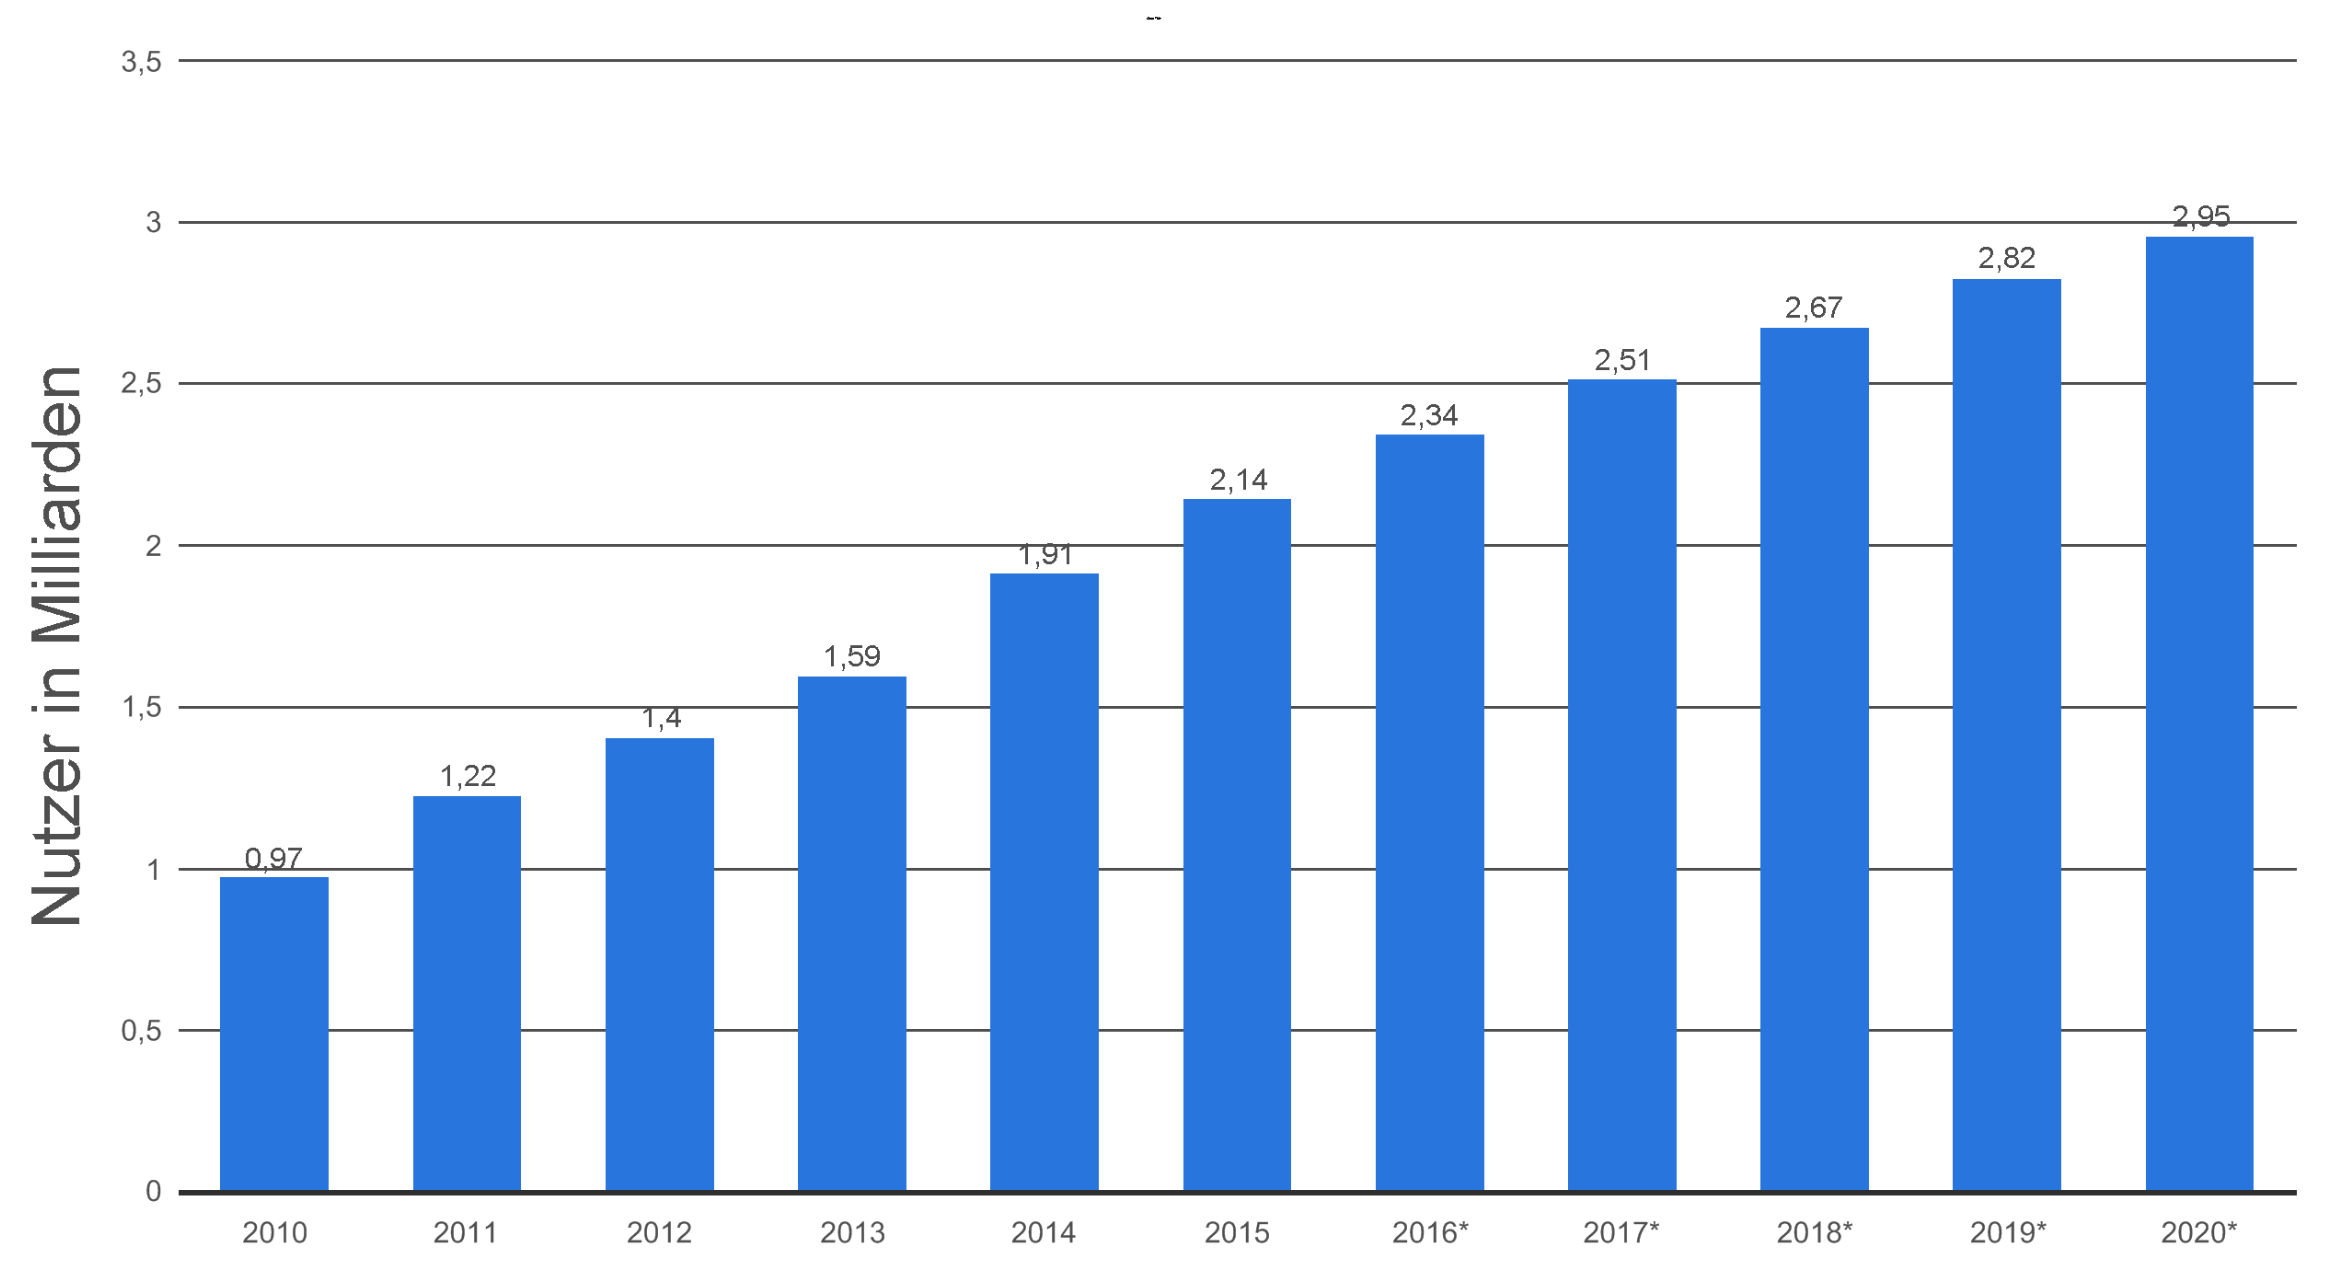
\includegraphics[scale=0.6]{resources/einf_02.png}
	\caption{Anzahl der Nutzer sozialer Netzwerke weltweit in den Jahren 2010
	bis 2015 sowie eine Prognose bis 2020 (in Milliarden)~\cite{statista-allg}.}
	\label{fig:overall}
\end{figure}

//hier noch etwas text. Uebergang von allg. zu Jugendlichen. evtl noch mehr statistiks

YouNow\footnote{\url{https://www.younow.com}} und
SnapChat\footnote{\url{https://www.snapchat.com}} sind zwei aufstrebende,
neuere Anwendungen in diesem Bereich und vor allem bei Kindern und Jugendlichen
sehr beliebt~\cite{statista-snapchat, vaterlaus2016snapchat}. Im Rahmen dieser Arbeit werden beide
etwas n\"aher betrachtet und auf m\"ogliche Gefahren in Bezug auf P\"adophilie
untersucht.
